As the statistics on punctuation and sentences tend to change between years (especially for the sentences lengths and number of commas), we tried to implement a metric with those statistics. \\

Those statistics are extracted for each year and combined in a single entry by year. For the metric, we take a sample of articles from one year, we merge them, as it was one big article, we compute the statistics on this article and we use a simple euclidean distance to compute the distance with each year. The result for a sample of 15 random articles from 1925 is observable in figure \ref{punct_metric_1925}.

\begin{figure}[H]
	\centering
    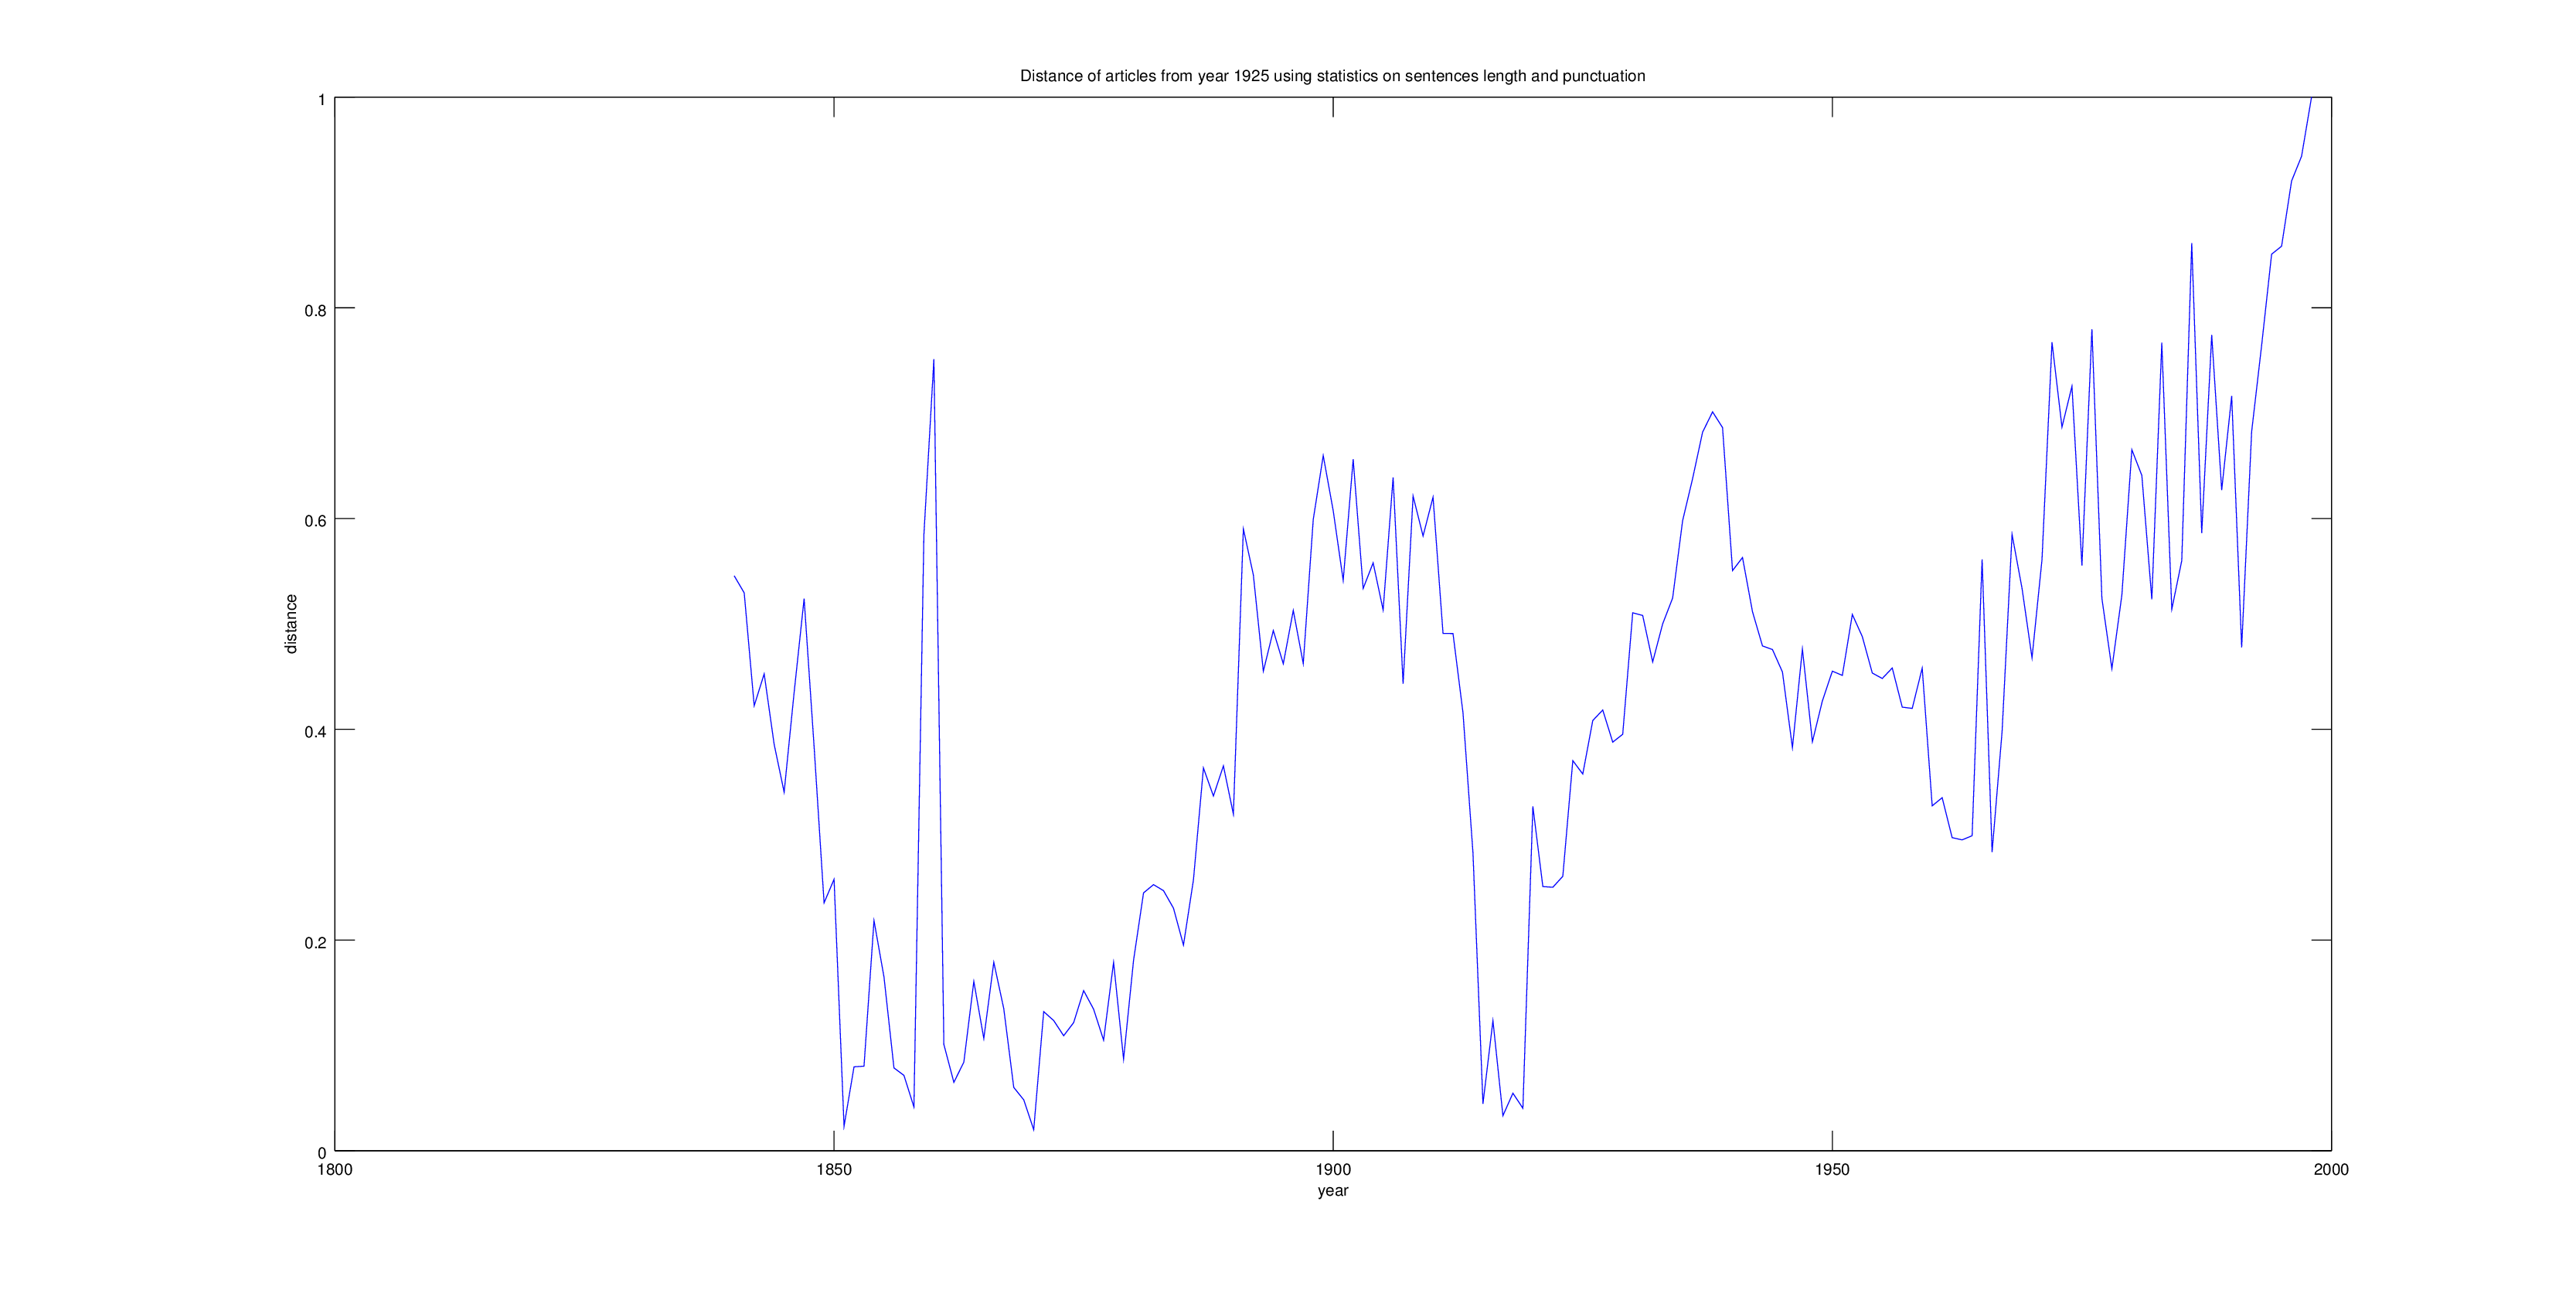
\includegraphics[scale=0.5]{Pictures/date_articles/punctuation/graph.png}
    \caption{Distance between a sample of 15 random articles from 1925 and each year}
    \label{punct_metric_1925}\hfill
\end{figure}

As we can see, it does not work that well, but with more time, we could have used machine learning methods instead of a simple euclidean distance, we think it could be useful to combine the result obtained them with other distances to enhance the classification.